\documentclass[ngerman,11pt]{article}

\usepackage[left=2.5cm, right=2.5cm, top=2cm, bottom=2cm]{geometry}
\usepackage{babel}
\usepackage{listings}
\usepackage{color}
\usepackage{hyperref}
\usepackage{csquotes}
\usepackage{awesomebox}
\MakeOuterQuote{"}

\pagenumbering{gobble}
\renewcommand{\lstlistingname}{Schnipsel}

% see overleaf
\definecolor{lightgray}{rgb}{0.95, 0.95, 0.95}
\definecolor{darkgray}{rgb}{0.4, 0.4, 0.4}
%\definecolor{purple}{rgb}{0.65, 0.12, 0.82}
\definecolor{editorGray}{rgb}{0.95, 0.95, 0.95}
\definecolor{editorOcher}{rgb}{1, 0.5, 0} % #FF7F00 -> rgb(239, 169, 0)
\definecolor{editorGreen}{rgb}{0, 0.5, 0} % #007C00 -> rgb(0, 124, 0)
\definecolor{orange}{rgb}{1,0.45,0.13}
\definecolor{olive}{rgb}{0.17,0.59,0.20}
\definecolor{brown}{rgb}{0.69,0.31,0.31}
\definecolor{purple}{rgb}{0.38,0.18,0.81}
\definecolor{lightblue}{rgb}{0.1,0.57,0.7}
\definecolor{lightred}{rgb}{1,0.4,0.5}

\definecolor{dkgreen}{rgb}{0,0.6,0}
\definecolor{gray}{rgb}{0.5,0.5,0.5}
\definecolor{mauve}{rgb}{0.58,0,0.82}

\lstdefinelanguage{CSS}{
    keywords={color,background-image:,margin,padding,font,weight,display,position,top,left,right,bottom,list,style,border,size,white,space,min,width, transition:, transform:, transition-property, transition-duration, transition-timing-function},
    sensitive=true,
    morecomment=[l]{//},
    morecomment=[s]{/*}{*/},
    morestring=[b]',
    morestring=[b]",
    alsoletter={:},
    alsodigit={-}
}

% JavaScript
\lstdefinelanguage{JavaScript}{
    morekeywords={typeof, new, true, false, catch, function, return, null, catch, switch, var, if, in, while, do, else, case, break},
    morecomment=[s]{/*}{*/},
    morecomment=[l]//,
    morestring=[b]",
    morestring=[b]'
}

\lstdefinelanguage{HTML5}{
    language=html,
    sensitive=true,
    alsoletter={<>=-},
    morecomment=[s]{<!-}{-->},
    tag=[s],
    otherkeywords={
        % General
        >,
        % Standard tags
        <!DOCTYPE,
        </html, <html, <head, <title, </title, <style, </style, <link, </head, <meta, />,
        % headings
        </h1, <h1, </h2, <h2, </ul, <ul, </ol, <ol, </li, <li, <img, </a, <a,
        % body
        </body, <body,
        % Divs
        </div, <div, </div>,
        % Paragraphs
        </p, <p, </p>,
        % scripts
        </script, <script,
        % More tags...
        <canvas, /canvas>, <svg, <rect, <animateTransform, </rect>, </svg>, <video, <source, <iframe, </iframe>, </video>, <image, </image>, <header, </header, <article, </article
    },
    ndkeywords={
        % General
        =,
        % HTML attributes
        charset=, src=, id=, width=, height=, style=, type=, rel=, href=,
        % SVG attributes
        fill=, attributeName=, begin=, dur=, from=, to=, poster=, controls=, x=, y=, repeatCount=, xlink:href=,
        % properties
        margin:, padding:, background-image:, border:, top:, left:, position:, width:, height:, margin-top:, margin-bottom:, font-size:, line-height:,
        % CSS3 properties
        transform:, -moz-transform:, -webkit-transform:,
        animation:, -webkit-animation:,
        transition:,  transition-duration:, transition-property:, transition-timing-function:,
    }
}

\lstdefinestyle{htmlcssjs} {%
% General design
%  backgroundcolor=\color{editorGray},
    basicstyle={\footnotesize\ttfamily},
    frame=b,
% line-numbers
    xleftmargin={0.75cm},
    numbers=left,
    stepnumber=1,
    firstnumber=1,
    numberfirstline=true,
% Code design
    identifierstyle=\color{black},
    keywordstyle=\color{blue}\bfseries,
    ndkeywordstyle=\color{editorGreen}\bfseries,
    stringstyle=\color{editorOcher}\ttfamily,
    commentstyle=\color{brown}\ttfamily,
% Code
    language=HTML5,
    alsolanguage=JavaScript,
    alsodigit={.:;},
    tabsize=2,
    showtabs=false,
    showspaces=false,
    showstringspaces=false,
    extendedchars=true,
    breaklines=true,
% German umlauts
    literate=%
        {Ö}{{\"O}}1
        {Ä}{{\"A}}1
        {Ü}{{\"U}}1
        {ß}{{\ss}}1
        {ü}{{\"u}}1
        {ä}{{\"a}}1
        {ö}{{\"o}}1
}

\lstset{frame=tb,
    language=Java,
    aboveskip=3mm,
    belowskip=3mm,
    showstringspaces=false,
    captionpos=b,
    columns=flexible,
    basicstyle={\small\ttfamily},
    numbers=left,
    numberstyle=\tiny\color{gray},
    keywordstyle=\color{blue},
    commentstyle=\color{dkgreen},
    commentstyle=\color{dkgreen},
    stringstyle=\color{mauve},
    breaklines=true,
    breakatwhitespace=true,
    tabsize=3,
    inputencoding=utf8
}

% Packages
\usepackage{amsmath}
\usepackage{graphicx}

% Document
\setlength{\parindent}{0pt}
\begin{document}

    {\huge \textbf{Websiten erstellen mit HTML und CSS}}

    \section{Die Idee}

    Jede Website, die wir uns im Internet anschauen, besteht aus einer \textit{Beschreibung},
    wie diese Website aussehen soll.
    Diese Beschreibung wird in \lstinline{HTML} \textit{(Hypertext Markup Language)}
    und \lstinline{CSS} \textit{(Cascading Stylesheets)} notiert.
    Der Browser (Chrome, Firefox, Safari,\dots) verwendet diese Beschreibung um die Website auf dem
    Bildschirm:

    \begin{center}
        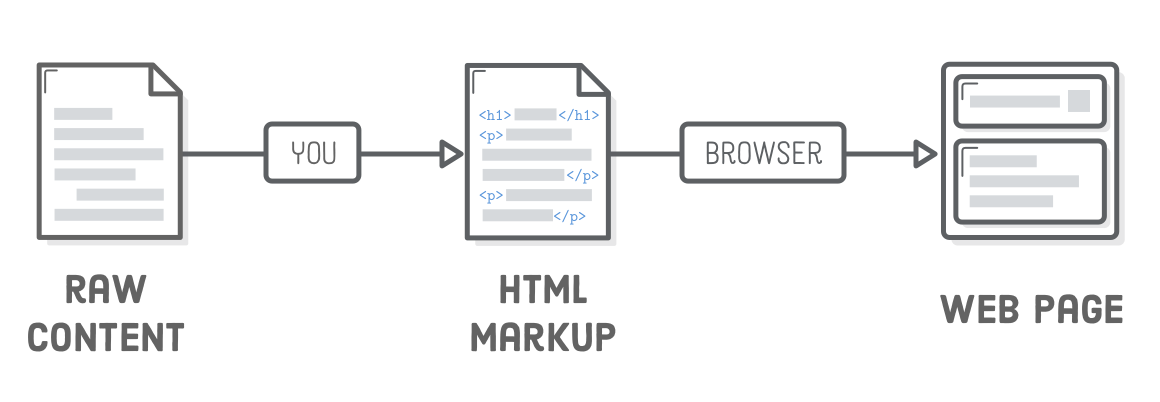
\includegraphics[width=0.6\textwidth]{code_to_website}
        \footnote{Bildquelle: \url{https://htmlcss.learn.uno/html-and-css/basic-web-pages/}}
    \end{center}

    Dabei dient \lstinline{HTML} der \textit{Strukturierung} unseres Seiteninhalts, während
    mit \lstinline{CSS} das Styling (also Farben, Größen, Animationen,\dots) definiert wird.

    \section{HTML - Inhalte Strukturieren}

    \lstinline{HTML} Code repräsentiert immer eine Baumstruktur (vgl.\ Baumdiagramm in Wahrscheinlichkeitsrechnung).
    Die \textit{Knoten} in diesem Baum sind \lstinline{HTML}-\textit{Elemente} und durch Verschachtelung der Elemente
    wird eine Eltern- / Kind-Beziehung hergestellt. \\

    Beispiel: \\

    \noindent\fbox{%
    \parbox{\textwidth}{%
        {\huge A very cool website} \\

        My christmas whishlist:
        \begin{itemize}
            \item A Ferrari
            \item Winning the lottery
            \item New books
        \end{itemize}
        \vspace{1cm}
        {\huge About me} \\

        Here is a very cool text about me.
    }%
    }\\

    \vspace{1cm}

    Wie ist dieser Inhalt sturkturiert?
    Wir haben zunächst eine äußere Box, das ist unsere "Wurzel" (\textit{root}-Element).
    Diese Box könnte zwei Kind-Elemente haben, ein Kind-Element für den oberen Absatz und eins
    für den unteren. \\

    Jeder der Absätze hätte wieder mehrere Kinder:
    Der obere Absatz ist unterteilt in 3 Kind-Elemente
    (die Überschrift, der Text zwischen Überschrift und der Liste und die Wunschliste)
    während der untere 2 hat (die Überschrift und der Text unterhalb Letzterer). \\

    Diese Strukturierung entspräche in etwa folgendem Baumdiagramm: \\

    \begin{center}
        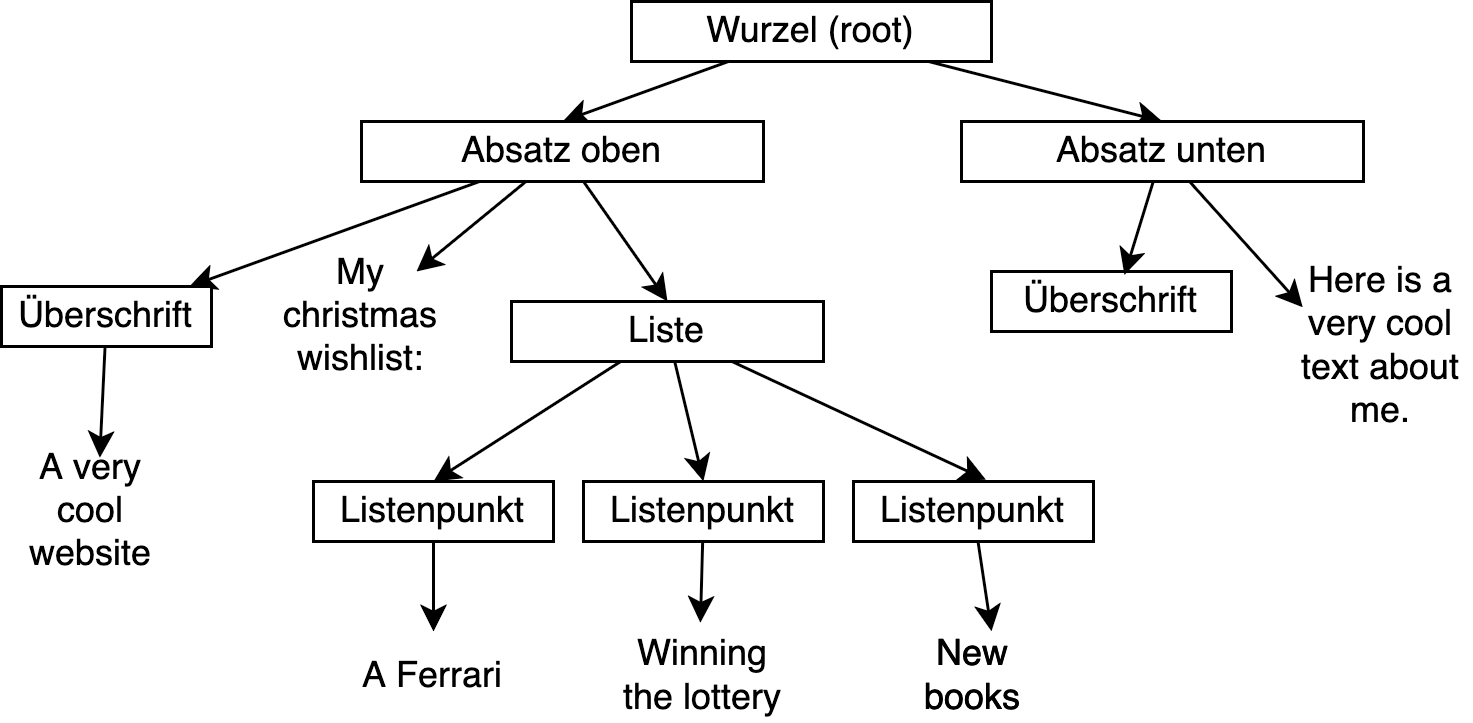
\includegraphics[width=0.6\textwidth]{html_tree}
    \end{center}


    In \lstinline{HTML} werden \textit{Elemente} durch \textit{Tags} repräsentiert.
    Es gibt Tags mit verschiedenen Bedeutungen und Funktionen, wir werden einige kennenlernen.
    Ein Tag hat immer einen \textit{Namen} und wird wie folgt notiert:

    \section{HTML - Grundlagen}

    \subsection{HTML Elemente}

    Die Knoten in oben beschriebenem Baumdiagramm sind in einem HTML Dokument
    die sogenannten HTML-Elemente.
    Ein Element wird wie folgt notiert:

    \begin{verbatim}<elementname>... inhhalt ...</elementname>\end{verbatim}

    "elementname" ist dabei der Name des Elements.
    Heißt das Element beispielsweise \verb_button_, so schreiben wir entsprechend \verb_<button>klick mich</button>_.

    Man nennt \verb_<...>_ das \textit{öffnende Tag} und \verb_</...>_ das \textit{schließende Tag} (man beachte das "/" in Letzterem).
    Alles was zwischen \verb_<...>_ und \verb_</...>_ steht, bildet den \textit{Inhalt} des Elements (die Kindknoten des Element-Knotens im Baumdiagramm). \\

    \tipbox{
        Jede Art von HTML-Element hat seine eigene \textit{Semantik}, also Bedeutung.
        Manche davon bringen bestimmte Funktionen oder Darstellungsarten mit sich, andere nicht -
        dennoch empfiehlt es sich den HTML-Code so zu schreiben, dass die Struktur, die dieser vorgibt,
        für den Leser (und sei es auch man selbst ein paar Tage später) einen \textit{Sinn} ergibt.
    }



    \subsection{Das HTML Grundgerüst}

    Jedem HTML-Dokument liegt folgendes Grundgerüst zugrunde:

    \begin{lstlisting}[style=htmlcssjs]
<!DOCTYPE>
<html>
    <head></head>
    <body>
        Eine tolle Seite
    </body>
</html>
    \end{lstlisting}

    Das \verb_<html>_ Element ist einfach die Wurzel des HTML Dokuments. \\
    Der \verb_<head>_ enthält Informationen \textit{über} die Seite (\textit{Metainformationen})
    und ist für uns zunächst nicht relevant. \\
    Der \verb_<body>_ repräsentiert den \textit{Inhalt} unseres HTML-Dokuments.
    Der gesamte Inhalt, alles was wir auf dieser Seite anzeigen wollen, kommt in den \verb_<body>_!

    \notebox{ {\verb(<!DOCTYPE>} ist ein spezielles Element. Es teilt dem Browser mit, dass die neueste
    HTML Version verwendet werden soll (HTML5). Lässt man es weg, können in manchen Browsern unerwartete Probleme auftauchen.}

    Wir wollen das Resultat nun im Browser betrachten:
    \begin{itemize}
        \item Tippe obigen HTML Code in einem beliebigen Text-Editor ein (beispielsweise VS-Code)
        \item Speichere die Datei unter dem Namen \lstinline{index.html}
        \item Navigiere zur gespeicherten Datei im Windows-Explorer und Doppelklicke diese (oder Rechtsklick $\rightarrow$ öffnen)
    \end{itemize}

    \notebox{Der Name der Datei ist eigentlich egal, die Endung \lstinline{.html} ist aber wichtig, weil der Browser sonst
    nicht versteht was er tun soll. Konventionell heißt die Startseite einer größeren Website \lstinline{index.html}.}

    \warningbox{Der Browser teilt uns nicht mit, wenn wir einen Fehler im HTML Code haben - er tut dann nur im Zweifel
    unerwartete Dinge. Vergessen wir beispielsweise das "/" in {\verb(</head>}, so sehen wir in manchen Browsern überhaupt nichts mehr.
    Daher empfiehlt es sich stets sorgfältig zu arbeiten und die vorgegebene Schreibweise stets zu befolgen.}

    \subsection{Verschiedene HTML Elemente}

    Wir tragen im Folgenden einige Beispiele von HTML Elementen zusammen. \\

    \verb_<p>_ --- steht für \textit{paragraph} (Absatz).
    Wird genutzt um Absätze zu unterteilen.
    Sorgt dafür, dass der Inhalt in einer neuen Zeile beginnt. \\

    Beispiel:

    \begin{lstlisting}[style=htmlcssjs]
<p>
    Ein toller Absatz!
</p>
<p>
    Ein weiterer toller Absatz!
</p>
    \end{lstlisting}

    \vspace{0.5cm}

    \verb_<h1>_ --- Definiert eine Überschrift der Ebene 1.
    Darüber hinaus gibt es \verb_<h2>_, \verb_<h3>_, \dots, \verb_<h6>_ für Überschriften
    niederer Ebenen. \\

    Beispiel:

    \begin{lstlisting}[style=htmlcssjs]
<h1>
    Rezeptesammlung
</h1>
<h2>
    Torten
</h2>
<h2>
    Kuchen
</h2>
    \end{lstlisting}

    \vspace{0.5cm}

    \verb_<ul>, <ol>_ --- Definiert eine ungeordnete (\textit{unordered}) oder geordnete (\textit{ordered}) Liste.
    Wird in Kombination mit \verb_<li>_ (\textit{list item}) verwendet, um Listen-ähnliche Inhalte zu strukturieren. \\

    Beispiel:

    \begin{lstlisting}[style=htmlcssjs]
<ul>
    <li>Atome</li>
    <li>Quarks</li>
    <li>Elektronen</li>
</ul>
<ol>
    <li>Aufschrauben</li>
    <li>Bauteil ersetzen</li>
    <li>Zuschrauben</li>
    <li>Testen</li>
</ol>
    \end{lstlisting}

    \vspace{0.5cm}

    \verb_<a>_ --- erzeugt einen Link, also Verweis auf eine andere Seite. \\

    Beispiel:

    \begin{lstlisting}[style=htmlcssjs]
<a href="https://www.google.de">klicke hier, um zu google zu gelangen</a>
    \end{lstlisting}

    \notebox{\lstinline{href} ist ein sogenanntes Attribut (siehe oben).
    Elemente können mehrere Attribute haben. \lstinline{href} steht für \textit{hyperreference} (Hyperverweis)
    und spezifiziert die "Zieladresse" für den Link. }

    \vspace{0.5cm}

    \verb_<img>_ --- für \textit{image}, wird verwendet um Bilder anzuzeigen. \\

    Beispiel:

    \begin{lstlisting}[style=htmlcssjs]
<img src="https://www.scinexx.de/wp-content/uploads/e/n/entenaugen_g.jpg"/>
    \end{lstlisting}

    \notebox{Der Wert des \lstinline{src}-Attributes (englisch \lstinline{source}: Quelle) ist die \textit{Adresse} (URL) zu einem Bild. Sehen wir ein Bild im Internet,
    können wir dessen Adresse meistens über \textit{Rechtsklick $\rightarrow$ Bildlink kopieren} (Bezeichnung kann variieren) kopieren.}

    \warningbox{Das {\verb_<img>} Element ist eine Ausnahme, was die Schreibweise angeht:
    Es gibt kein schließendes Tag {\verb_</img>}, sondern das Tag schließt quasi sich selbst - ein sogenanntes selbtschließendes Tag.
    Solche Elemente können keine Kindknoten haben.
    }

    \vspace{1cm}

    Eine gute Übersicht über alle verfügbaren HTML-Elemente gibt es beispielsweise hier: \\
    \url{https://developer.mozilla.org/de/docs/Web/HTML/Element}

    \newpage

    \section{CSS - Grundlagen}

    Mit HTML alleine können wir das \textit{Aussehen} der einzelnen Elemente nur begrenzt beeinflussen.
    Zum Beispiel setzt der Browser automatisch verschiedene Schriftgrößen für Überschrift-Elemente (\verb_<h1>, <h2>, ..._),
    für ein schönes individuelles Design reicht das aber natürlich nicht aus. \\

    CSS besteht aus einer Reihe von \textit{Eigenschaften}, die bestimmte \textit{Werte} annehmen können.
    Weisen wir einem Element eine Eigenschaft mit einem bestimmten Wert zu, beeinflussen wir damit die Erscheinung des Elements. \\

    Beispiel: Die CSS Eigenschaft \verb_color_ beeinflusst die \textit{Schriftfarbe} eines Elements (und seiner Kindelemente).
    \verb_color_ können wir als Wert - offensichtlich - eine Farbe zuweisen.

    Farben können in CSS auf verschiedene Arten angegeben werden:

    \begin{itemize}
        \item Als englischer Name (red, green, fuchsia, navy, maroon, crimson und viele mehr -
        eine Aufschlüsselung gibt es hier: \url{https://developer.mozilla.org/de/docs/Web/CSS/named-color})
        \item Als \textit{Hexadezimalzahl}: z.B. \verb_#FA2355_
        \item Als Komposition in verschiedenen Farbräumen, bspw. \verb_rgb(r, g, b)_, \verb_hsv(h, s, v)_ und weitere
    \end{itemize}

    \subsection{Inline-CSS}

    Eine Möglichkeit, Elementen Werte für CSS Eigenschaften zuzuweisen, ist über sogenanntes \textit{Inline-CSS}.
    Dazu verwendet man das Element-Attribut \textit{style}, und schreibt alle Eigenschaften und deren Werte in den Wert
    dieses Attributs: \verb_<element style="eigenschaft1: wert1; eigenschaft2: wert2; ...">...</element>_.
    Eigenschaft und Wert trennt man mit einem Doppelpunkt (:), verschiedene Eigenschaften mit einem Semikolon (;). \\

    Beispiel:

    \begin{lstlisting}[type=htmlcssjs]
<p style="color: blue">
    Das ist ein wunderbarer Absatz mit blauem Text.
</p>
    \end{lstlisting}

    \subsection{Eine Reihe von CSS Eigenschaften}

    \begin{itemize}
        \item \verb_color_ --- Schriftfarbe, Wert ist eine Farbe
        \item \verb_background_ --- Hintergrund, Wert ist Farbe, Hintergrundbild oder Gradient
        \item \verb_font-size_ --- Schriftgröße, Wert ist eine Größenangabe (s.u.)
        \item \verb_font-family_ --- Schriftart, Wert ist Name einer Schriftart
        \item \verb_border-color_ --- Farbe des Rahmens um das Element
        \item \verb_border-width_ --- Größe des Rahmens um das Element
        \item \verb_border-style_ --- Typ des Rahmens um das Element, der Wert ist eines von \lstinline{none, hidden, dotted, dashed, solid, double, groove, ridge, inset, outset}
        \item \verb_margin_ --- der Abstand von der Außenkante des Elements zu anderen Elementen, Wert ist eine Größenangabe
        \item \verb_padding_ --- der Abstand von der Innenkante des Elements zu seinem Inhalt, Wert ist eine Größenangabe
    \end{itemize}

    \notebox{Viele CSS Eigenschaften beeinflussen die Größe von Dingen. Größenangaben in CSS kann man in verschiedenen
    Einheiten machen: Pixel (\lstinline{px}), Punkt (\lstinline{pt}), Centi- und Millimeter (\lstinline{cm, mm}) und viele weitere.
    Einen Größen-Wert gibt man an mit \lstinline{[zahl][einheit]}, also zum Beispiel \lstinline{15px}.
        }

    \notebox{Wann immer der Wert für eine Eigenschaft ein Name ist (zum Beispiel für eine Farbe oder eine Schriftart), müssen wir
    Anführungszeichen verwenden. Zum Beispiel: \lstinline{color: "orange"} oder \lstinline{font-family: "Calibri"}.}

    \section{Aufgaben}

    \subsection{Steckbrief}

    Entwerfe mit HTML und CSS einen ausführlichen Steckbrief über eine Person des öffentlichen Lebens oder eine imaginäre Person.
    Nutze alle dir bekannten HTML Elemente und CSS Stile, experimentiere mit der Darstellung und tausche dich für Inspiration
    mit deinen Mitschülern aus.

\end{document}
